\section{More Complex Formulas}
The formulas in the previous section are common formulas, but are fairly simple. The benefit of using temporal logics is that a wide variety of behaviours can be expressed, including propositions about the robot \textit{and} about the workspace. Up to now, we have not looked at any formulas that include atomic propositions about potential tasks. We will show through examples that the same ideas presented in the previous chapter still hold true for this complex tasks, and show the speed up we get by using our algorithm compared to the accepted algorithm. 

\subsection{Example 1}
We look at the example from \cite{guo15} which says "eventually pick up the red ball. Once it is done, move to one basket and drop it. At last come back to room one and stay there". This task can be written as the LTL formula $\varphi = \diamond (\text{rball} \wedge \diamond \text{basket}) \wedge \diamond \square r1$. The B\"uchi automaton corresponding to this formula as translated by \cite{gastin01} is shown in figure \ref{fig:buchiEx1}

\begin{figure}[!htb]
\centering
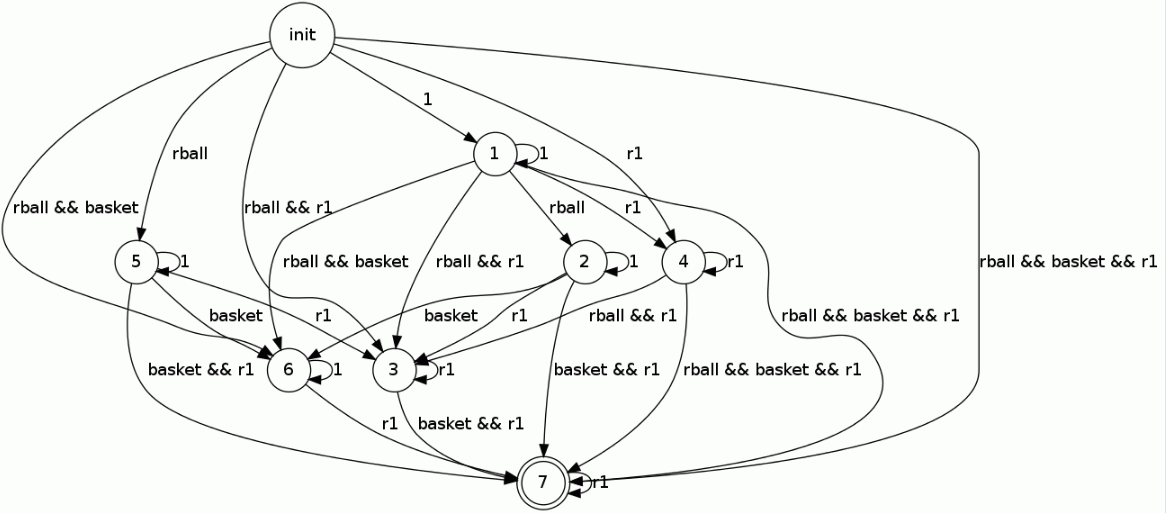
\includegraphics[scale=0.4]{buchiEx1}
\label{fig:buchiEx1}
\caption{B\"uchi Automaton Corresponding to $\varphi = \diamond (\text{rball} \wedge \diamond \text{basket}) \wedge \diamond \square r1$}
\end{figure} 


As we can see, there are many edges in this automaton and edges that have \&\& in the label. These paths can only be taken if we satisfy both of the propositions at the same time. However, because in our example the propositions do not overlap (the ball is not in the same room as the basket, and the neither the ball or basket is located in room 1) these edge are impossible to take. Therefore we remove these edges from the automaton (show the code for this). We then have a much simpler automaton that is shown in figure \ref{fig:ex1SimplifiedBuchi}

\begin{figure}
\centering
\begin{tikzpicture}[->,>=stealth',shorten >=1pt,auto,node distance=2.8cm,
                    semithick]
  \tikzstyle{every state}=[fill=red,draw=black,text=black]

  \node[initial,state] (A)                    {$q_1$};
  \node[state] (B)                    [right of=A]{$q_2$};
  \node[state] (C)                    [right of=B]{$q_4$};
  \node[state] (E)                    [above of=B]{$q_3$};
  \node[state] (F)                    [above of=C]{$q_5$};
  \node[state,accepting]         (D) [right of=C] {$q_6$};

  \path (A) edge              node {rball} (B)
  		%(A) edge [loop above] node {$\neg \pi_1$} (A)
  		(B) edge [loop below] node {$\neg$ basket} (B)
  		(B) edge              node {basket} (C)
  		(A) edge              node {$\neg$rball} (E)
  		(E) edge              node {rball} (F)
  		(F) edge              node {basket} (C)
  		(C) edge [loop below] node {$\neg r1$} (C)
  		(C) edge              node {$r1$} (D)
  		(E) edge [loop above] node {$\neg$rball} (E)
  		(F) edge [loop above] node {$\neg$basket} (F)
  		(D) edge [loop above] node {$r1$} (D);
\end{tikzpicture}
\caption{Simplified B\"uchi Automaton for $\varphi = \diamond (\text{rball} \wedge \diamond \text{basket}) \wedge \diamond \square r1$ 1}
\label{fig:ex1SimplifiedBuchi}
\end{figure} 

In this automaton, we can see that $d(q_1)=3$, $d(q_2)=2$, $d(q_3)=3$, $d(q_4)=1$, $d(q_5)=2$, $d(q_6)=0$. We can also see that from the illustration of the workspace, that the ball (rball) is not located next to the initial node, so the first proposition must be $\neg$rball. Examining the automaton in figure \ref{fig:ex1SimplifiedBuchi} that then we are guaranteed to go to a node $q_1' = \langle \pi_i , q_3 \rangle$ on the first step. This means that we will never go to a node with the projection of $q_2$. Therefore we are in the same situation as for sequencing i.e.\ there is only on sequence of actions that will satisfy the formula, implying that our algorithm will find the same path as the accepted algorithm, just much faster. 

\subsection{Example 1 Overlapping Regions}
We now look at the same example, except now we have a different workspace. We choose this example to show what happens if the regions of interest are overlapping. We show multiple scenarios. First, if rball is with the basket. If this is the case, then rball and basket can be satisfied simultaneously. Therefore we have to admit paths with rball \&\& basket into the automaton. The automaton is now
\begin{figure}
\centering
\begin{tikzpicture}[->,>=stealth',shorten >=1pt,auto,node distance=3.5cm,
                    semithick]
  \tikzstyle{every state}=[fill=red,draw=black,text=black]

  \node[initial,state] (A)                    {$q_1$};
  \node[state] (B)                    [right of=A]{$q_2$};
  \node[state] (C)                    [right of=B]{$q_4$};
  \node[state] (E)                    [above of=B]{$q_3$};
  \node[state] (F)                    [above of=C]{$q_5$};
  \node[state,accepting]         (D) [right of=C] {$q_6$};

  \path (A) edge              node {rball} (B)
  		(A) edge   [bend right=90]	 node {rball \&\& basket} (C)
  		(E) edge					node {rball \&\& basket} (C)
  		%(A) edge [loop above] node {$\neg \pi_1$} (A)
  		(B) edge [loop below] node {$\neg$ basket} (B)
  		(B) edge              node {basket} (C)
  		(A) edge              node {$\neg$rball} (E)
  		(E) edge              node {rball} (F)
  		(F) edge              node {basket} (C)
  		(C) edge [loop below] node {$\neg r1$} (C)
  		(C) edge              node {$r1$} (D)
  		(E) edge [loop above] node {$\neg$rball} (E)
  		(F) edge [loop above] node {$\neg$basket} (F)
  		(D) edge [loop above] node {$r1$} (D);
\end{tikzpicture}
\caption{Simplified B\"uchi Automaton Corresponding to $\varphi = \diamond (\text{rball} \wedge \diamond \text{basket}) \wedge \diamond \square r1$ 2}
\label{fig:ex1OverlapSimplifiedBuchi}
\end{figure} 

In this automaton, we now have $d(q_1)=2$, $d(q_2)=2$, $d(q_3)=2$, $d(q_4)=1$, $d(q_5) = 2$ and $d(q_6)=0$. We see again that rball and basket are not one step away from the initial node, implying that we cannot take the first step rball or rball \&\& basket. This means that we cannot ever go to $q_2$.

\subsection{Example 2}
We now look at the example \cite{guo15} in which the robot has to pick up and deliver two different balls (rball and gball) to two different baskets, and the robot cannot carry two balls at once. After delivering both balls, the robot is to go to r1 and stay there. This task is formalized as $\varphi = \diamond (\text{rball} \wedge \diamond (\text{basket} \wedge \text{r2})) \wedge \diamond(\text{gball} \wedge \diamond (\text{basket} \wedge \text{r4})) \wedge \square (\text{rball} \rightarrow \textbf{X}(\neg \text{gball} \U \text{basket})) \wedge \square (\text{gball} \rightarrow \textbf{X} (\neg \text{rball} \U \text{basket})) \wedge \diamond \square \text{r1}$